\documentclass[crop=false, class=memoir]{standalone}
\usepackage[utf8]{inputenc}%Nødvendig for danske bogstaver
\usepackage[danish]{babel}%Sørger for at ting LaTeX gør automatisk er på dansk
\usepackage{csquotes}
\usepackage{geometry}%Til opsætning af siden
\geometry{lmargin = 2.5cm,rmargin = 2.5cm}%sætter begge magner
\usepackage{lipsum}%Fyldtekst, til brug under test af layoutet
\usepackage{float}
\usepackage{graphicx}%Tillader grafik
\usepackage{epstopdf}%Tillader eps filer
\usepackage{marginnote}% Noter i margen
\interfootnotelinepenalty=10000 %undgår at fodnoter bliver spilittet op.
\usepackage[sorting=none]{biblatex}
\addbibresource{litteratur.bib}
\usepackage[hidelinks]{hyperref}%Tillader links
\usepackage{subcaption} % Tillader underfigurer
\usepackage[font={small,sl}]{caption}	% Caption med skrå tekst ikke kursiv

\usepackage{xcolor} %Bruges til farver
\usepackage{forloop} %Bruges til nemmere for loops

\newcounter{opgave}[chapter] %Definerer opgavenumrene og hvornår de nulstilles
\renewcommand{\theopgave}{\thechapter.\arabic{opgave}} %Definerer udseende af opgavenummereringen
\newcounter{delopgave}[opgave] %Definerer delopgavenumrene
\newcounter{lvl} %Definerer en "variabel" til senere brug

\definecolor{markerColor}{rgb}{0.0745098039, 0.262745098, 0.584313725} %Definerer farven af markøren
\newcommand{\markerSymbol}{\ensuremath{\bullet}} %Definerer tegnet for markøren
\newlength{\markerLength} %Definerer en ny længde
\settowidth{\markerLength}{\markerSymbol} %Sætter den nye længde til bredden af markøren

\newenvironment{opgave}[2][0]{%Definerer det nye enviroment, hvor sværhedsgraden er den første parameter med en default på 0
\newcommand{\opg}{\refstepcounter{delopgave}\par\vspace{0.1cm}\noindent\textbf{\thedelopgave)\space}}%Definerer kommando til delopgave
\refstepcounter{opgave}%Forøger opgavenummer med 1 og gør den mulig at referere til
\setcounter{lvl}{#1}%Sætter "variablen" lvl lig med angivelsen af sværhedsgraden
\noindent\hspace*{-0.75em}\hspace*{-\value{lvl}\markerLength}\forloop{lvl}{0}{\value{lvl}<#1}{{\color{markerColor}\markerSymbol}}\hspace*{0.75em}%Sætter et antal af markører svarende til sværhedsgraden
\textbf{Opgave \theopgave : #2}\newline\nopagebreak\ignorespaces}{\bigskip} %Angiver udseende af titlen på opgaverne samt mellemrummet mellem opgaver



\usepackage{mathtools}%Værktøjer til at skrive ligninger
\renewcommand{\phi}{\varphi}%Vi bruger varphi
\renewcommand{\epsilon}{\varepsilon}%Vi bruger varepsilon
\usepackage{physics}%En samling matematikmakroer til brug i fysiske ligninger
\usepackage{braket}%Simplere kommandoer til bra-ket-notation
\usepackage{siunitx}%Pakke der håndterer SI enheder godt
\DeclareSIUnit\clight{\text{\ensuremath{c}}} % Lysets fart i vakuum som c og ikke c_0
\usepackage{chemmacros}
\usechemmodule{isotopes}
\usepackage{tikz}
\usepackage[danish]{cleveref}
\usepackage{nicefrac}
% \renewcommand{\ref}[1]{\cref{#1}}
\creflabelformat{equation}{#2(#1)#3}
\crefrangelabelformat{equation}{#3(#1)#4 to #5(#2)#6}
\crefname{equation}{ligning}{ligningerne}
\Crefname{equation}{Ligning}{Ligningerne}
\crefname{section}{afsnit}{afsnitene}
\Crefname{section}{Afsnit}{Afsnitene}
\crefname{figure}{figur}{figurene}
\Crefname{figure}{Figur}{Figurene}
\crefname{table}{tabel}{tabellerne}
\Crefname{table}{Tabel}{Tabellerne}
\crefname{opgave}{opgave}{opgaverne}
\Crefname{opgave}{Opgave}{Opgaverne}
\crefname{delopgave}{delopgave}{delopgaverne}
\Crefname{delopgave}{Delopgave}{Delopgaverne}

\newcommand{\eqbox}[1]{\begin{empheq}[box=\fbox]{align}
	\begin{split}
	#1
	\end{split}
\end{empheq}}

\newcommand{\kb}{\ensuremath{k_\textsc{b}}}

\DeclareSIUnit{\parsec}{pc}
\DeclareSIUnit{\lightyear}{ly}
\DeclareSIUnit{\astronomicalunit}{AU}
\DeclareSIUnit{\year}{yr}
\DeclareSIUnit{\solarmass}{M_\odot}
\DeclareSIUnit{\solarradius}{R_\odot}
\DeclareSIUnit{\solarluminosity}{L_\odot}
\DeclareSIUnit{\solartemperature}{T_\odot}
\DeclareSIUnit{\earthmass}{M_\oplus}
\DeclareSIUnit{\earthradius}{R_\oplus}
\DeclareSIUnit{\jupitermass}{M_J}

% Infobokse og lignende
% http://mirrors.dotsrc.org/ctan/graphics/awesomebox/awesomebox.pdf
% \usepackage{awesomebox}


% Egen infobokse (virker kun med begrænsede symboler)

\usepackage[framemethod=tikz]{mdframed}
\usetikzlibrary{calc}
\usepackage{kantlipsum}

\usepackage[tikz]{bclogo}

\tikzset{
    % lampsymbol/.style={scale=2,overlay}
    % lampsymbol/.pic={\centering\tikz[scale=5]\node[scale=10,rotate=30]{\bclampe}}.style={scale=2,overlay}
    infosymbol/.style={scale=2,overlay}
}

\newmdenv[
    hidealllines=true,
    nobreak,
    middlelinewidth=.8pt,
    backgroundcolor=blue!10,
    frametitlefont=\bfseries,
    leftmargin=.3cm, rightmargin=.3cm, innerleftmargin=2cm,
    roundcorner=5pt,
    % skipabove=\topsep,skipbelow=\topsep,
    singleextra={\path let \p1=(P), \p2=(O) in ($(\x2,0)+0.92*(1.1,\y1)$) node[infosymbol] {\bcinfo};},
    % singleextra={\path let \p1=(P), \p2=(O) in ($(\x2,0)+0.5*(2,\y1)$) node[infosymbol] {\bcinfo};},
]{info}

% Skal bruges som
% \begin{info}[frametitle={Titel}]
%     Tekst
% \end{info}
\usepackage{import}
\begin{document}
\chapter{Speciel Relativitetsteori} \label{chap:rel_facit}




\begin{opgave}{Det Galileiske Relativitetsprincip}{1}
	Det Galileiske Relativitetsprincip siger, at Newtons bevægelseslove er ens i alle inertielle referencesystemer.\\
	Vi forestiller os nu et tog, der kører med en konstant hastighed $v$ ift. sporet. En passager i toget tager så en sten og slipper den fra hvile.  
	\opg Brug Galileis relativitetsprincip til at beskrive stenens bevægelse set fra en observatør i toget.\\
	
	Da toget bevæger sig med konstant hastighed, er det et inertialsystem. Vi ved, at en sted falder lodret ned mod jorden i et inertialsystem, der er i hvile, og derfor må den også gøre det i toget. Newtons bevægelseslove er jo ens i alle inertialesystemer.\\  
	\opg Brug Galilei-transformationen (3.1) til at give en beskrivelse af stenens bevægelse set fra en observatør på Jorden.\\
	
	Lad $x$-aksen pege i den retning, som toget kører. Da stenen falder lodret nedad i toget, vil $x'=0$ for alle tider $t$ og $t'$. Fra Galilei-transformationen for $x'$ får man da at:
	
	$$0 = x-vt \quad \Rightarrow \quad x = vt$$
	
	Stenen falder altså ikke lodret ned set fra Jorden, da den har fået en vertikal hastighed på $v$. 
\end{opgave}

\begin{opgave}{Kombination af Galileiske transformationer}{1}	
	To tog kører parallelt med hinanden i $x$-retningen, det ene med hastighed $V$ og det andet med hastighed $U$,
	relativt til jorden. Lad det første tog være $S'$ og det andet $S''$, med deres respektive koordinater. Jorden betegnes $S$.
	\opg Hvad er den Galileiske transformation fra $S \left( x,y,z,t \right)$ til $S'' \left( x'',y'',z'',t'' \right)$?\\
	
	Her bruger man formlerne for de Galileiske transformationer (3.1). Man får at:
	
	$$t''=t$$
	$$x''=x-Ut$$
	$$y''=y$$
	$$z''=z$$
	\opg Hvad er den Galileiske transformation fra $S'$ til $S''$?\\

	Her bruger man formlerne for de Galileiske transformationer (3.1). Man får at:
	
	$$t''=t'$$
	$$y''=y'$$
	$$z''=z'$$
	
	For at finde transformationen for $x''$, kan man først finde transformationen for $x'$. Den er fra (3.1): $x' = x - Vt $. Så kan man løse for $x$, hvilket giver: $x = x' + Vt$. Dette kan man så indsætte i udtrykket for $x''$, hvor man får:
	
	$$x'' = x-Ut = x' + Vt -Ut = x' - \left( U - V \right)t = x' - \left( U-V \right)t'$$
	
	hvor det er brugt at $t=t'$.\\
	\opg Hvad svarer størrelsen $\left( U- V \right)$ til?\\
	

	$U-V$ er $S''$ systemets hastighed relativt til $S'$ systemet.	 
\end{opgave}

\begin{opgave}{Løbetur i Regnvejr}{1}
	En dag hvor det regner, falder dråberne lodret ned med $\SI{2}{m/s}$. En person løber vandret af sted med $\SI{3}{m/s}$. Ved hvilken vinkel ift. vandret skal personen holde sin paraply for bedst muligt at skærme for regnen? (hint: Kig på regndråbernes bevægelse set fra løberens referencesystem).\\
	
	Set fra løberens referencesystem falder regnen ikke lodret ned, da det har både en lodret hastighed ($\SI{2}{m/s}$) og en vandret hastighed ($\SI{3}{m/s}$). Kigger man på dråbens fald over $\SI{1}{s}$, vil dråben bevæge sig langs hypotenusen i en trekanten nedenfor:
	\begin{center}
	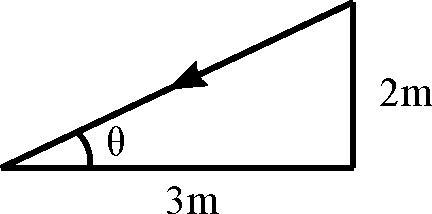
\includegraphics[scale=0.9]{Rel/regn_fig.pdf}	
	\end{center}
	
	Man finder da $\theta$:
	
	$$\theta = \arctan \left( \frac{2}{3} \right) = 33.69^\circ$$	
\end{opgave}

\begin{opgave}{Flyvetur i Blæsevejr}{1}
	En flyvemaskine kan flyve med  $\SI{500}{km/t}$, og der er en vindhastighed på $\SI{200}{km/t}$ fra vest mod øst.
	\opg Flyets pilot styrer flyet mod nord. I hvilken retning bevæger flyet sig, og hvad er flyets hastighed set fra en observatør på Jorden, som betegnes $S$? (hint: Kig på et referencesystem $S'$, der bevæger sig med vinden og benyt hastighedstransformationerne (3.2) til at oversætte flyets bevægelse i dette system til $S$).\\
	
	Lad $y$-aksen pege mod nord og $x$-aksen pege mod øst. Lad videre $x$- og $x'$-aksen være parallelle, og de to systemers origoer være sammenfaldende for $t=t'=0$. Kigger man på flyet fra $S'$, vil der ikke være nogen vind. Derfor flyver flyet direkte nord på set fra dette system. Det må betyde, at flyets hastigheder i de forskellige retninger er:
	
	$$u'_y = \SI{500}{km/t} \quad \quad \text{og} \quad \quad u'_x = u'_z = 0$$
	
	\vspace{2mm}
	
	Kigger man på (3.2) får man da at $u_y = u'_y$ og $u_z = u'_z$. For $u_x$ får man:
	
	$$u'_x = 0 = u_x - v \quad \Rightarrow \quad u_x = v = \SI{200}{km/t}$$
	
	\vspace{2mm}
	
	da $v$ jo er vindens hastighed her. For at finde den retning som flyet flyver i, set fra Jorden, kan man kigge på flyets bevægelse over 1 time:
	
	\begin{center}
		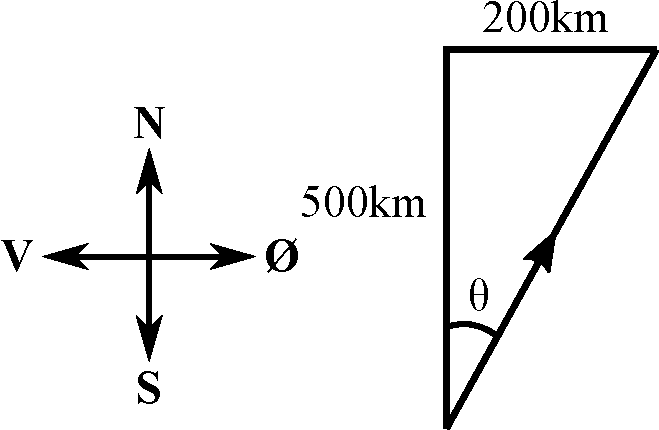
\includegraphics[scale=0.8]{Rel/fly_fig.pdf}
	\end{center}
	
	Så findes $\theta$:
	
	$$\theta = \arctan \left( \frac{200}{500} \right) = 21.80^\circ$$
	
	\vspace{2mm}
	
	Og Flyets hastighed set fra Jorden findes vha. Pythagoras:
	
	$$v_{\text{fly}} = \sqrt{500^2 + 200^2} \, \si{km/t} = \SI{538.52}{km/t} $$
	\opg I hvilken retning skal piloten styre, hvis flyet skal flyve mod nord? Hvad er flyets hastighed set fra en observatør på Jorden i dette tilfælde?\\
	
	Hvis flyet skal flyve mod nord, er det nødt til at have en hastighed $u_x = - \SI{200}{km/t}$. Igen får man en trekant:
	
	\begin{center}
		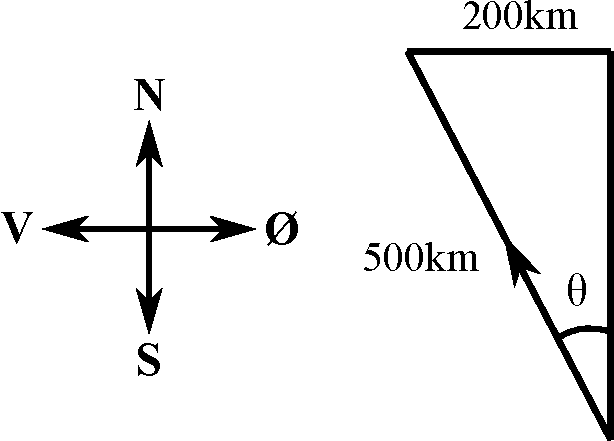
\includegraphics[scale=0.8]{Rel/fly_fig2.pdf}
	\end{center}

	Man kan finde $\theta$:
	
	$$\sin \theta = \frac{\SI{200}{km}}{\SI{500}{km}} \quad \Rightarrow \quad \theta = \arcsin \left( \frac{200}{500} \right) = 23.58^\circ$$
	
	Og hastigheden bliver:
	
	$$v_{\text{fly}} = \sqrt{500^2 - 200^2} \ \si{km/t} = \SI{458.26}{km / t}$$
\end{opgave}

\begin{opgave}{Flodræset}{2}
	En flod er $\SI{20}{m}$ bred og vandet i floden strømmer af sted med en hastighed på $\SI{1}{m/s}$. To svømmere Arthur og Barbara arrangerer et ræs. Arthur skal svømme $\SI{20}{m}$ ned af floden og tilbage, mens Barbara skal svømme lige over floden og tilbage. Både Arthur og Barbare kan svømme med $\SI{2}{m/s}$.
	\opg I hvilken retning skal Barbara svømme, for at hun kommer lige over floden?\\
	
	Set fra et referencesystem der bevæger sig med strømmen, skal Barbaras hastighed opad være $\SI{1}{m/s}$ og hendes totale hastighed $\SI{2}{m/s}$. Man kan lave en trekant, og finde at Barbara skal svømme med en vinkel $\theta$ ift. en lige linje over floden. Vinklen er:
	
	$$\theta = \arcsin \left( \frac{1}{2} \right) = 30.0^\circ$$
	\opg Hvem vinder ræset og med hvor meget?\\
	
	Kald bredten af floden for $L$. Barbara er praktisk talt nød til at svømme en længere tur. Længden hun svømmer hver vej er givet:
	
	$$\cos \theta = \frac{L}{L_{\text{Bar}}} \quad \quad \Rightarrow \quad \quad L_{\text{Bar}} = \frac{L}{\cos \theta}  $$
	
	\vspace{2mm}
	
	For Barbara tager hele turen altså:
	
	$$t_{\text{Bar}} = \frac{2 \cdot L_{\text{Bar}}}{\SI{2}{m/s}} = \frac{2 \cdot \SI{20}{m}}{\cos \left( 30.0^\circ \right) \cdot \SI{2}{m/s}} = \SI{23.09}{s}$$
	
	\vspace{2mm}
	
	For Arthur kan man regne tiden for hver af de to ture:
	
	$$t_{\text{Art,ned}} = \frac{\SI{20}{m}}{\SI{3}{m/s}} = \SI{6.667}{s}$$
	
	$$t_{\text{Art,op}} = \frac{\SI{20}{m}}{\SI{1}{m/s}} = \SI{20}{s}$$
	
	\vspace{2mm}
	
	Det giver:
	
	$$t_{\text{Art}} = t_{\text{Art,ned}} + t_{\text{Art,op}} = \SI{26.667}{s}$$
	
	\vspace{2mm}
	
	Barbara vinder altså ræset.
\end{opgave}


\begin{opgave}{Hvornår er relativitetsteori virkelig nødvendig?}{1}
	Som det ses, så indgår $\gamma$ meget ofte i relativitetsteori. Når $\gamma$ væsentligt større end 1, er det
	nødvendigt at bruge de relativistiske udtryk, frem for de Galileiske. For hvilken hastighed (i enheder af $c$) er
	værdien af $\gamma$:
	\opg 1\% større end 1?
	\opg 10\% større end 1?
	\opg 100\% større end 1?\\
	
	Her kan man opskrive følgende:
	
	$$x = \frac{1}{\sqrt{1- v^2/c^2}} \quad \Rightarrow \quad \frac{v}{c} = \sqrt{1- \frac{1}{x^2}}$$
	
	
	\noindent
	Så kan man ellers bare indsætte $1.01$, $1.10$ og $2.00$ på $x$'s plads, hvorved man finder at:
	
	$$\gamma = 1.01 \quad \Rightarrow \quad \frac{v}{c} = 0.1404 $$
	$$\gamma = 1.10 \quad \Rightarrow \quad \frac{v}{c} = 0.4166 $$
	$$\gamma = 2 \quad \Rightarrow \quad \frac{v}{c} = 0.8660 $$
\end{opgave}

\begin{opgave}{Et lille tankeeksperiment}{1}
	De relativistiske effekter ses ikke i hverdagen, fordi $c$ er så stor, sammenlignet med hastigheder vi oplever i
	hverdagen. Men hvad nu hvis lysets hastighed var meget mindre? Lad os se hvad der sker, hvis nu $c = 50$
	km/t.
	\opg Usain Bolts topfart er $44,72 \si{km/t}$. Hans hvilemasse er $94 \si{kg}$. Hvad er hans masse, når han når
	topfart?\\
	
	Her bruger man (3.25), der giver den relativistiske masse. Det giver at:
	
	$$m_{\text{rel}} = \frac{\SI{94}{kg}}{\sqrt{1- (\SI{44.72}{km/t})^2 / (\SI{50}{km/t})^2}} =  \SI{210.2}{kg} $$
\end{opgave}

\begin{opgave}{Muoner i Jordens atmosfære}{1}
	Muoner er ustabile sub-atomare partikler, der med en levetid på $2,2 \,\mu\si{\s}$ $(2,2 \cdot 10^{-6} \si{s})$ henfalder til elektroner.
	Muoner produceres omkring $10 \si{km}$ over Jordens overflade, hvor energirige partikler fra rummet rammer
	atmosfæren, og de rejser med en hastighed tæt på lysets i forhold til Jorden, lad os sige $v = 0,999c$.
	\opg Hvad er den længste afstand en muon kan nå at rejse i sin levetid på $2,2 \,\mu\si{\s}$?\\
	
	Den er givet som:
	
	$$L = v \cdot T_0 = 0.999 \cdot 3.00 \times 10^8 \ \si{m/s} \cdot 2.2 \times 10^{-6} \ \si{s} = \SI{659.34}{m}$$
	\opg Fra ovenstående lader det til, at muonerne aldrig vil nå os på overfladen. Ikke desto mindre detekterer vi
	dem! Men levetiden angivet er i muonens hvilesystem. Hvad er dens levetid målt for en observatør på
	Jorden?\\
	
	Levetiden som målt af en observatør på Jorden er givet ved:
	
	$$T=\gamma T_0=\frac{2.2 \times 10^{-6}\si{s}}{\sqrt{1-0.999^2}}=49.2058 \times 10^{-6}\si{s}=49.2058\mu\si{s} $$
	\opg Hvor langt vil muonen nå nu?\\
	
	Mounen når nu en længde på 
	$$L=v \cdot T=0.999 \cdot 3.00 \times 10^8 \si{m/s} \cdot 49.2058 \times 10^{-6} = 14746.98 \si{m} = 14.74698 \si{km}$$
	\opg Fra muonens synspunkt lever den stadig kun $2,2 \, \mu\si{\s}$. Hvad er tykkelsen af $10 \si{km}$ atmosfære, set fra
	muonens system?\\
	
	Set fra mounens system, vil atmosfæren have en tykkelse på
	$$L=\frac{L_0}{\gamma}=10000 \si{m} \cdot \sqrt{1-0.999^2} = 447.102 \ \si{m}$$
\end{opgave}

\begin{opgave}{Relativitet og rumfart}{1}
	For nyligt valgte NASA at pensionere deres rumfærger. Indtil da var rumfærgen en forholdsvis billig måde at
	fragte udstyr og mennesker ud i rummet, fordi færgen og det meste af det man brugte til at sende den op med
	kunne genanvendes. Efter endt mission kunne rumfærgen lande som et fly.\\
	\indent
	En observatør på Jorden måler en landingsbane til at være $3600 \si{m}$. En rumfærge befinder sig i kredsløb om
	Jorden med en hastighed af $4,00 \cdot 10^7 \si{m/s}$ relativt til Jorden. Vi antager, at dens bane er en ret linje under hele
	opgaven, og at den flyver parallelt med landingsbanen.
	\opg Hvad er længden af landingsbanen målt af piloten på rumfærgen?\\
	
	Længden af landingsbanen som målt af piloten er
	$$L=\frac{L_0}{\gamma}=3600 \si{m} \cdot \sqrt{1-\frac{16.00 \times 10^{14} \si{m/s}}{9.00 \times 10^{16} \si{m/s}}} = 3567.86 \si{m}$$
	\opg En observatør på Jorden måler tiden der går, fra rumfærgen er direkte over den ene ende af landingsbanen,
	og til den er over den anden ende. Hvor lang tid får vedkommende?\\
	
	Tiden er givet ved strækning divideret med hastigheden,
	$$t=\frac{3600 \si{m}}{4.00 \times 10^7 \si{m/s}} = 9 \times 10^{-5} \si{s}$$
	\opg Piloten på rumfærgen måler den tid, det tager ham at flyve længden af landingsbanen. Hvilken værdi får
	han?\\
	
	Denne opgave kan løses på to måder. Vi kan enten benytte os af den forkortede længde og bruge samme metode som tidligere,
	$$t=\frac{3567.86 \si{m}}{4.00 \times 10^7 \si{m/s}}=89.1965 \cdot 10^{-6} \si{s}$$
	
	Alternativt kan man udregne tiden ved at benytte sig af længdeforkortelse, hvor tiden målt fra rumfærgen er $T_0$,
	$$T_0=\frac{T}{\gamma}=9 \times 10^{-5} \si{s} \cdot \sqrt{1-\frac{16.00 \times 10^{14} \si{m/s}}{9.00 \times 10^{16} \si{m/s}}}=89.1965 \cdot 10^{-6} \si{s}$$
	\opg Rumfærgen har en vægt på godt $2000$ tons. Hvad ville rumfærgen veje, hvis en observatør på Jorden
	kunne veje den, mens den var i kredsløb, dvs. hvad er dens relativistiske masse?\\
	
	Rumfærgens relativistiske masse er givet ved
	$$m_{\text{rel}}=\gamma m=\frac{2.00 \times 10^6}{\sqrt{1-\frac{16.00 \times 10^{14} \si{m/s}}{9.00 \times 10^{16} \si{m/s}}}}=2.018 \times 10^6 \si{kg}$$
	\opg Rumfærgen er $60$ meter lang og $10$ meter høj i dens eget referencesystem. Hvor lang og høj er rumfærgen
	for en observatør på Jorden?\\
	
	Højden vil ikke ændre sig, da længdeforkortelse kun har en effekt i bevægelsesretningen. Længden som målt af en observatør på Jorden er
	$$L=\frac{L_0}{\gamma}=60 \si{m} \cdot \sqrt{1-\frac{16.00 \times 10^{14} \si{m/s}}{9.00 \times 10^{16} \si{m/s}}}=49.464 \si{m}$$
\end{opgave}

\begin{opgave}{Tvillinge-Paradokset - Her skal du bruge hovedet}{2}
	Tvillinge-paradokset er et af de mest kendte paradokser inden for speciel relativitetsteori. Egentligt er det ikke
	et paradoks, da Einstein allerede løste det tilbage i 1905. I denne opgave skal I også løse det. Det kræver, at man
	lige tænker sig lidt om.
	
	Barbara og Arthur er tvillinger. Arthur bliver på Jorden, mens Barbara rejser af sted med et rumskib, med
	hastighed nær $c$. På et tidspunkt vender rumskibet hurtigt, og flyver tilbage til Jorden. Da Barbara kommer
	tilbage, mødes hun med Arthur til en sammenligning. For Arthur har Barbara rejst ud og hjem igen med nær
	lysets hastighed. Derfor er tiden for hende gået langsommere, og hun vil derfor se yngre ud end Arthur. Men
	fra Barbaras synspunkt er det jo Arthur, som har bevæget sig i forhold til hende. Derfor bruger hun samme
	argument til at konkludere, at han vil se yngre ud end hende. Samtidigt er der jo ikke noget referencesystem,
	som er bedre end andre, så et argument der bygger på dette vil komme frem til, at alle resultater må være
	symmetriske mellem de to tvillinger. De er altså lige gamle.
	\opg Ud fra ovenstående lader det til, at der er tre muligheder, men kun en kan være rigtig. Hvilken mulighed
	er det?\\
	
	Svaret ligger i at Barbaras rumskib bliver nød til at accelerere, når det vender for at flyve tilbage til jorden. Barbaras referencesystem vil altså ikke være et inertielt referencesystem, og den specielle relativitetsteori, vil derfor ikke gælde for hende. Det betyder således at problemet ikke er symmetrisk set fra de to tvillinger, og det rigtige svar er derfor, at Barbara er yngre end Arthur.\\
	\opg Hvis en af tvillingerne er ældst, kan du så sige noget om, hvor lang tid der er gået for den yngste i
	forhold til den ældste?\\
	
	Tiden der er gået for den ældste tvilling er $T$. Vi kan så bruge formlen for tidsforlængelse til at finde den tid der er gået for den yngste,
	$$T_0=T \cdot \sqrt{1-\frac{v^2}{c^2}}$$
\end{opgave}


\begin{opgave}{Lorentz-transformationens udledelse}{2}
	I afsnit 3.7 udledte vi Lorentz-transformationen. I ligning 3.15 så vi på højresiden, hvor vi konkluderede at $x$'s koefficient skulle være 1, og herved fandt frem til gamma-funktionen $\gamma$. Vi var dog ikke helt færdig med udledelsen i dette tilfælde.
	\opg I skal nu færdiggøre udledelsen af Lorentz-transformationen, ved at undersøge om højresiden af ligning 3.15 stemmer overens med ligning 3.11, når vi kender $\gamma$.\\
	
	Vi søger i denne opgave at omskrive højresiden af 3.15, $c^2\gamma^2t^2-\gamma^2v^2t^2$, ved hjælp af $\gamma$ funktionen, således at det stemmer overens med højresiden af 3.11, $c^2t^2$.
	\begin{align*}
		&c^2\gamma^2t^2-\gamma^2v^2t^2 \\
		&\downarrow \\
		&c^2t^2\gamma^2(1-v^2/c^2) \\
		&\downarrow \\
		&c^2t^2\frac{1}{1-v^2/c^2} \\
		&\downarrow \\
		&c^2t^2
	\end{align*}
\end{opgave}

\begin{opgave}{Lorentz-transformationen på differens-form}{2} \label{lorentz_diff2}
	Lad os betragte to begivenheder $P_1$ og $P_2$, som i inertialsystemet $S$ har koordinaterne $(x_1,y_1,z_1,t_1)$ og $(x_2,y_2,z_2,t_2)$. Svarende hertil har vi de fire koordinatdifferencer
	\begin{align}
		\Delta t=t_2-t_1, \	 \Delta x=x_2-x_1, \ \Delta y=y_2-y_1, \ \Delta z= z_2-z_1 \nonumber
	\end{align}
	\opg I skal nu finde de tilsvarende størrelser,
	\begin{math}
		\Delta t',  \Delta x',  \Delta y',  \Delta z'
	\end{math}
	i inertialsystemet $S'$, som bevæger sig i forhold til $S$ med hastigheden $v$, ved hjælp af Lorentz-transformationen.\\
	
	Da vi har $\Delta t=t_2-t_1$, må den tilsvarende differens i $S'$ være $\Delta t'=t'_2-t'_1$. Vi kan herved finde et udtryk for denne differens ved at bruge Lorentz-transformationen,
	\begin{align*}
		\Delta t'=\gamma(t_2-vx_2/c^2)-\gamma(t_1-vx_1/c^2)=\gamma(t_2-t_1-vx_2/c^2+vx_1/c^2)=\gamma(\Delta t-v\Delta x/c^2)
	\end{align*}
	Man gør det samme for de tre andre størrelser:
	$$\Delta x' = \gamma \left( x_2 - vt_2 \right) - \gamma \left( x_1 - vt_1 \right) = \gamma \left( x_2 - x_1 -vt_2 + vt_1 \right) = \gamma \left( \Delta x - v \Delta t \right)$$
	
	$$\Delta y' = y'_2 - y'_1 = y_2 - y_1 = \Delta y \quad \quad \text{og} \quad \quad \Delta z' = z'_2 - z'_1 = z_2 - z_1 = \Delta z$$
\end{opgave}

\begin{opgave}{Tidsforlængelse og Længdeforkortelse vha. Lorenz-transformationen}{2}
	I denne opgave skal I prøve at udlede formlen for tidsforlængelse og længdeforkortelse vha. Lorentz-transformationen. Det gøres ved at kigge på en proces set fra to referencesystemer $S$ og $S'$ i standardkonfigurationen. Processens start og slutning i tid og rum beskrives ved $(x_1,t_1)$ og $(x_2,t_2)$ i $S$ og $(x'_1,t'_1)$ og $(x'_2,t'_2)$ i $S'$.
	\opg Udtrykket for $\Delta t'$ I fandt i opgave \ref{lorentz_diff2} indeholder både $t_1,t_2$ og $x_1,x_2$. Hvad må man kræve omkring processens start-- og slutkoordinater $x_1$ og $x_2$ i $S$, for at udtrykket bliver lig udtrykket for tidsforlængelse?\\
	
	Man må kræve at $x_1=x_2$, således at man har $\Delta t'=\gamma(\Delta t-v \cdot 0/c^2)=\gamma\Delta t$.\\
	\opg Forklar hvorfor kravet fra 1) sikre, at vi kigger på en "ren" tidsforlængelse, hvor rum og tid ikke bliver blandet sammen.\\
	
	I tilfældet af at $\Delta t' =\gamma\Delta t$, kan vi se at tiden $\Delta t'$ kun afhænger af den relative hastighed og tidsforskellen $\Delta t$ i $S$. Hvis vi ikke krævede at $\Delta x=0$, ville udtrykket afhænge både af de forrige variable og begivenhedernes position.\\
	\opg Forklar hvordan udtrykket for $\Delta t'$ fra opgave \ref{lorentz_diff2}, hvis man ikke bruger kravet fra 1), viser at rum og tid bliver blandet sammen i relativitetsteori.\\
	
	Se opgave 13.2.\\
	\opg Gennemgå de samme trin som I har gjort ovenfor, denne gang hvor I kigger på længdeforkortelse. Start derfor med $\Delta x'$, og undersøg hvad man må kræve omkring $t_1$ og $t_2$.\\
	
	I dette tilfælde vil $\Delta x'$ være hvilelængden. For at udtrykket for $\Delta x'$ skal stemme overens med udtrykket for længdeforkortelse, må vi kræve at $t_1=t_2$, således at vi har
	\begin{align*}
	&\Delta x'=\gamma(\Delta x-v*0) \\
	&\downarrow \\
	&\Delta x=\frac{\Delta x'}{\gamma}
	\end{align*}
	
	Vi ser her igen at kravet om at $\Delta t = 0$ resulterer i en "ren" længdeforkortelse, da udtrykket kun afhænger af den relative hastighed $v$ og hvilelængden $\Delta x'$.
\end{opgave}

\begin{opgave}{Cæsars død og Kristi fødsel}{2}
	Cæsar blev myrdet år 44 f.Kr., og afstanden fra Rom til Betlehem kan sættes til 2300 km.
	\opg Findes der nogen iagttager, for hvem Cæsars død og Kristi fødsel er samtidige? Hvorfor/hvorfor ikke?\\
	
	Vi skal i denne opgave bruge den tidslige Lorentz-transformationen på differensform. Man kan så opstille to inertialsystemer $S$ og $S'$, hvor $S'$ bevæger sig med hastigheden $v$ i forhold til $S$. For at de to begivenheder sker samtidigt skal $\Delta t'=0$, og man kan herved opstille en ligning og isolere den nødvendige hastighed $v$.
	\begin{align*}
		&0=\gamma(\Delta t-v\Delta x/c^2) \\
		&\downarrow \\
		&0=\frac{\Delta t-v\Delta x/c^2}{\sqrt{1-v^2/c^2}} \\
		&\downarrow \\
		&0=\Delta t-v\Delta x/c^2 \\
		&\downarrow \\
		&\frac{\Delta tc^2}{\Delta x}=v
	\end{align*}
	Vi indsætter de opgivet størrelser og udregner hastigheden,
	\begin{align*}
		v=\frac{1387584000 s \cdot (3.00\cdot 10^8)}{2300000 m}=5.430 \times 10^{19}  \ \si{m/s}
	\end{align*}
	Vi kan herved konkludere at der ikke findes nogen iagttager, for hvem Cæsars død og Kristi fødsel er samtidige, da den nødvendige hastighed er langt større end lysets hastighed.
\end{opgave}

\begin{opgave}{Samtidighed}{2}
	To begivenheder har i inertialsystemet $S$ koordinaterne $(t_1,x_1,y_1,z_1)=(L/c,L,0,0)$ og $(t_2,x_2,y_2,z_2)=(L/2c,2L,0,0)$.
	\opg Der findes et inertialsystem, $S'$, i hvilket disse begivenheder er samtidige. Find hastigheden af $S'$ i forhold til $S$.\\
	
	I denne opgave skal vi benytte os af det samme udtryk som vi kom frem til i den forrige opgave. Denne gang er $\Delta t=\frac{L}{2c}-\frac{L}{c}=\frac{Lc}{2c^2}-\frac{Lc}{c^2}=-\frac{L}{2c}$ og $\Delta x=2L-L=L$. Dette indsættes, og et udtryk for hastigheden udregnes,
	\begin{align*}
		v=-\frac{\frac{L}{2c}c^2}{L}=-\frac{\frac{Lc}{2}}{L}=-\frac{Lc}{2L}=-\frac{c}{2}
	\end{align*}
	\opg Hvad er den fælles tidskoordinat, $t'$, for disse begivenheder i $S'$?\\
	
	Da vi nu kender hastigheden $v$, kan vi finde et udtryk for den fælles tidskoordinat $t'$ for de to begivenheder ved at bruge den tidslige Lorentz-transformation,
	\begin{align*}
		&t'=\gamma(\frac{L}{c}+\frac{cL}{2c^2}) \\
		&\downarrow \\
		&t'=\gamma(\frac{2L}{2c}+\frac{L}{2c}) \\
		&\downarrow \\
		&t'=\gamma\frac{3L}{2c} \\
		&\downarrow \\
		&t'=\sqrt{\frac{4}{3}}\frac{3}{2}\frac{L}{c} \\
		&\downarrow \\
		&t'=\sqrt{\frac{4}{3}}\sqrt{\frac{9}{4}}\frac{L}{c} \\
		&\downarrow \\
		&t'=\sqrt{3}\frac{L}{c}
	\end{align*}
\end{opgave}

\begin{opgave}{En stangs hastighed}{2}
	En stang med hvilelængde $l_0$ bevæger sig med jævn hastighed i sin længderetning. Set fra $S$ tager det tiden $\tau$ for stangen at passere et fast punkt i $S$. 
	\opg Find stangens hastighed som en brøkdel af lysets hastighed, $c$?\\
	
	Ved brug af længdeforkortnings formlen, er stangens længde i $S$ givet ved $L=L_0\sqrt{1-v^2/c^2}$. Herudover kan vi beskrive længden i $S$ ved $L=v\tau$. Vi kan herved bruge disse to udtryk til at finde stangens hastighed,
	\begin{align*}
		&v\tau=L_0\sqrt{(1-v^2/c^2)} \\
		&\downarrow \\
		&v^2\tau^2=L_0^2(1-v^2/c^2) \\
		&\downarrow \\
		&v^2\frac{\tau^2}{L_0^2}=1-v^2/c^2 \\
		&\downarrow \\
		&\frac{v^2}{c^2}(\frac{\tau^2}{L_0^2}+1)=1 \\
		&\downarrow \\
		&\frac{v}{c}=\frac{1}{\sqrt{\frac{\tau^2}{L_0^2}+1}}
	\end{align*}
\end{opgave}

\begin{opgave}{Invarians af lyspuls bevægelse}{2}
	Et referencesystem $S'$ bevæger sig i $x$-retningen med hastigheden $v$ relativt til et andet referencesystem $S$. Til tiden $t'=t=0$ krydser de to referencesystemer hinanden (deres origo er samme sted), og i netop dette øjeblik udsendes en lyspuls fra origo i $S'$. Efter en tid $t'$ er lyspulsens afstand $x'$ i $S'$ givet ved $x'^2 = c^2 t'^2$. 
	\opg Vis at afstanden $x$ i $S$ er givet ved $x^2 = c^2 t^2$ (hint: Brug Lorentz transformationerne).\\
	
		Vi benytter os her af den Lorentz-transformationen for $t'$ og $x'$:
	\begin{align*}
	&\gamma^2(x-vt)^2=c^2\gamma^2(t-vx/c^2)^2 \\
	&\downarrow \\
	&x-vt=c \cdot (t-vx/c^2) \\
	&\downarrow \\
	&x+vx/c=ct+vt \\
	&\downarrow \\
	&x(1+v/c)=ct(1+v/c) \\
	&\downarrow \\
	&x=ct \\
	&\downarrow \\
	&x^2=c^2t^2		
	\end{align*} 
\end{opgave}

\begin{opgave}{Referencesystemer - samme sted og samme tid}{3}
	To begivenheder er observeret i et referencesystem $S$ og kan beskrives ved $\left( x_1 , t_1 \right)$ og $\left( x_2 , t_2 \right)$. Et andet referencesystem $S'$ bevæger sig langs $x$-aksen med en hastighed $v$, således at de to begivenheder sker samme sted på $x$-aksen set fra $S'$.
	\opg Vis at tidsforskellen $\Delta t'$ mellem begivenhederne i $S'$ er givet ved:
	$$\Delta t' = \sqrt{\left( \Delta t \right)^2 - \left( \frac{\Delta x}{c} \right)^2}$$
	(hint: Brug $x'_1 = x'_2$ og Lorentz-transformationerne).\\
	
	$t_1'=t_2'$ og Lorentz-transformationen bruges først til at opstille et udtryk for hastigheden $v$,
	\begin{align*}
	&x_1-vt_1=x_2-vt_2 \\
	&\downarrow \\
	&\Delta x=v \cdot \Delta t \\
	&\downarrow \\
	&v=\frac{\Delta x}{\Delta t} \\
	\end{align*}
	
	Herefter bruger vi Lorentz-transformationen på $\Delta t'=t_2'-t_1'$,
	\begin{align*}
	&\Delta t'=\gamma(t_2-vx_2/c^2)-\gamma(t_1-vx_1/c^2) \\
	&\downarrow \\
	&\Delta t'=\frac{\Delta t-\frac{v\Delta x}{c^2}}{\sqrt{1-\frac{v^2}{c^2}}} \\
	&\downarrow \\
	&\Delta t'=\frac{\Delta t - \frac{\Delta x^2}{\Delta t^2c^2}}{\sqrt{1-\frac{\Delta x^2}{\Delta t^2c^2}}}
	&\downarrow \\
	&\Delta t'=\frac{\Delta t - \frac{\Delta x^2}{\Delta t^2c^2}}{\sqrt{1-\frac{\Delta x^2}{\Delta t^2c^2}}} \cdot \frac{\sqrt{\Delta t^2}}{\sqrt{\Delta t^2}} \\
	&\downarrow \\
	&\Delta t'=\frac{\Delta t^2-\frac{\Delta x^2}{c^2}}{\sqrt{\Delta t^2-\frac{\Delta x^2}{c^2}}} \\
	&\downarrow \\
	&\Delta t' = \sqrt{\Delta t^2-\frac{\Delta x^2}{c^2}}
	\end{align*}
	\opg Brug ovenstående resultat til at vise, at såfremt $\Delta x > c \Delta t$, så vil der ikke eksistere et referencesystem $S'$, hvor begivenhederne sker samme sted.\\
	
	Vi indser først at $\Delta x^2 > c^2\Delta t^2$ er det samme som $\Delta x > c\Delta t$. Vi kan så omskrive det forrige udtryk til
	$$\Delta t'=\sqrt{\frac{c^2\Delta t^2-\Delta x^2}{c^2}}$$
	Hvis $\Delta x^2 > c^2\Delta t^2$ er gældende, vil $\Delta t'$ være imaginært. Medmindre du er Stephen Hawking, så er imaginær tid udefineret.\\
	\opg Hvis $\Delta x > c \Delta t$, så findes der i stedet et andet referencesystem $S'$, hvor de to begivenheder sker samtidigt. Vis at afstanden $\Delta x'$ mellem de to begivenheder i dette referencesystem er givet ved:
	$$\Delta x' = \sqrt{\left( \Delta x \right)^2 - c^2 \left( \Delta t \right)^2}$$
	(hint: Brug $t'_1 = t'_2$ og Lorentz-transformationerne).\\
	
	$t_1'=t_2'$ benyttes til at udregne hastigheden $v$,
	\begin{align*}
	&t_1-x_1v/c^2=t_2-x_2v/c^2 \\
	&\downarrow \\
	&\Delta t=\frac{\Delta x v}{c^2} \\
	&\downarrow \\
	&v=\frac{c^2\Delta t}{\Delta x}
	\end{align*}
	Herefter bruger vi Lorentz-transformationen på $\Delta x'= x_2'-x_1'$,
	\begin{align*}
	&\Delta x'=\gamma(\Delta x-v\Delta t)=\frac{\Delta x-v\Delta t}{\sqrt{1-\frac{v^2}{c^2}}} \\
	&\downarrow \\
	&\Delta x'=\frac{\Delta x-\frac{c^2\Delta t^2}{\Delta x}}{\sqrt{1-\frac{c^2\Delta t^2}{\Delta x^2}}} \\
	&\downarrow \\
	&\Delta x'=\frac{\Delta x-\frac{c^2\Delta t^2}{\Delta x}}{\sqrt{1-\frac{c^2\Delta t^2}{\Delta x^2}}} \cdot \frac{\sqrt{\Delta x^2}}{\sqrt{\Delta x^2}} \\
	&\Delta x'=\frac{\Delta x^2-c^2\Delta t^2}{\sqrt{\Delta x^2-c^2\Delta t^2}} = \sqrt{\Delta x^2-c^2\Delta t^2}
	\end{align*}
	\opg Brug ovenstående resultat til at vise, at såfremt $c \Delta t > \Delta x$, så vil der ikke eksistere et referencesystem $S'$, hvor begivenhederne sker samtidigt.\\
	
		Ligesom i 18.2, så er $c^2\Delta t^2 > \Delta x^2$ ækvivalent med $c\Delta t > \Delta x$. I tilfældet af at $c^2\Delta t^2 > \Delta x^2$ er gældende, vil $\Delta x'$ ikke være reel.
\end{opgave}


I de følgende to opgaver, vil det være nødvendigt at kigge på funktioner af to variable, og hvordan sådanne funktioner ændre sig, når begge variable ændre sig på samme tid. 
Forestil jer, at  vi har en funktion $z$, der afhænger både af $y$ og $x$. Dette skriver man typisk $z=f \left( x,y \right)$. Hvis man har en ændring $\Delta x$ samt en ændring $\Delta y$ kan man approksimere ændringen $\Delta z$ på følgende måde:

$$\Delta z \approx \dv{z}{x} \cdot \Delta x + \dv{z}{y} \cdot \Delta y$$


Såfremt man lader ændringerne $\Delta x$ og $\Delta y$ gå mod nul, vil ovenstående ikke længere være en approksimation, og man skriver at:

$$dz = \dv{z}{x} \cdot dx + \dv{z}{y} \cdot dy$$


hvor $dz$, $dy$ og $dx$ er infinitesimale (meget små) versioner af $\Delta z$, $\Delta y$ og $\Delta x$.\\

\begin{opgave}{Lorentz-transformationen for hastighed}{2}
	I denne opgave skal i prøve at udlede Lorentz-transformationen for hastighed. Dette kan gøres ved at finde et udtryk for $dx'$ og $\dd{t'}$, som det er beskrevet ovenfor. Da $dx'$ og $\dd{t'}$ vil være de øjeblikkelige ændringer i $x'$ og $t'$, må det derfor gælde at $v'_x = dx'/\dd{t'}$.\\
	
	Som det første bruger man at:
	
	$$dx' = \dv{x'}{x} \cdot dx + \dv{x'}{t} \cdot dt = \frac{dx - v dt}{\sqrt{1- v^2 / c^2}} $$
	
	$$\dd{t'} = \dv{t'}{x} \cdot dx + \dv{t'}{t} \cdot dt = \frac{dt - v dx/c^2}{\sqrt{1- v^2 / c^2}}  $$
	
	Så finder man $v'_x$ ved at dividere disse:
	
	$$v'_x = dx'/\dd{t'} = \frac{\gamma (dx - v dt)}{\gamma (dt - v dx/c^2)} = \frac{dx - v dt}{dt - v dx/c^2} = \frac{dx/dt - v}{1 - v dx/dtc^2} = \frac{v_x - v}{1 - v v_x / c^2} $$
\end{opgave}

\begin{opgave}{Lorentz-transformationen for acceleration}{3}
	Lad $S'$ være et referencesystem der bevæger sig med hastighed $v$ i forhold til et andet referencesystem $S$. Et objekt bevæger sig relativt i forhold til $S$ langs $x$-aksen med en øjeblikkelig hastighed $v_x$ og øjeblikkelig acceleration $a_x$. Målet med de følgende trin er at finde et udtryk for accelerationen $a'_x$ i referencesystemet $S'$.
	\opg Find et udtryk for $\dd{t'}$.\\
	
	Dette findes som i forrige opgave.
	
	$$\dd{t'} = \dv{t'}{x} \cdot dx + \d{t'}{t} \cdot dt = \frac{dt - v dx/c^2}{\sqrt{1- v^2 / c^2}}  $$
	\opg Find et udtryk for $dv'_x$.\\
	
	Da $v'_x$ kun afhænger af en variabel $v_x$ finder man at:
% 	\begin{align*}
% 	dv'_x = \d{v'_x}{v_x} \cdot dv_x = \left( \d{\left( v_x - v \right)}{v_x}  \cdot \frac{1}{1-vv_x/c^2} + \d{\frac{1}{1-vv_x/c^2}}{v_x} \cdot (v_x-v) \right) dv_x  \\
% 	=  \left( \frac{1}{1-vv_x/c^2} + \frac{vv_x/c^2 - v^2/c^2}{\left( 1-vv_x/c^2 \right)^2} \right) dv_x = \left( \frac{1-vv_x/c^2}{\left( 1-vv_x/c^2 \right)^2} + \frac{vv_x/c^2 - v^2/c^2}{\left( 1-vv_x/c^2 \right)^2} \right) dv_x \\
% 	= \left( \frac{1-v^2/c^2}{\left( 1 - vv_x/c^2 \right)^2} \right) dv_x \\
% 	\end{align*}
	
	Før det sidste trin er det værd at sikre jer, at i har fået de rigtige resultater. I skulle gerne have fundet at:
	$$\dd{t'} = \gamma \left( dt - v dx / c^2 \right)$$
	$$dv'_x = \left( \frac{1 - v^2/c^2}{ \left( 1-vv_x/c^2 \right)^2 } \right) dv_x$$
	\opg Brug at $a'_x = dv'_x / \dd{t'}$, $a_x = dx/dt$ samt at $v_x = dx/dt$ til at vise, at $a'_x$ er givet ved:
	$$a'_x = a_x \left( 1- \frac{v^2}{c^2} \right)^{3/2}  \left( 1 - \frac{vv_x}{c^2}  \right)^{-3}$$
	
	Her dividerer man de to udtryk med hinanden.
	
	$$ a'_x = dv'_x/\dd{t'} = dv_x \frac{ (1 - v^2/c^2)/ \left( 1-vv_x/c^2 \right)^2}{\gamma \left( dt - v dx / c^2 \right)} = \frac{dv_x}{dt} \frac{ (1 - v^2/c^2)/ \left( 1-vv_x/c^2 \right)^2}{\gamma \left( 1 - v dx /dt c^2 \right)} $$
	
	$$ = a_x \frac{ (1 - v^2/c^2)/ \left( 1-vv_x/c^2 \right)^2}{\gamma \left( 1 - v v_x/ c^2 \right)} = a_x \left( 1- \frac{v^2}{c^2} \right)^{3/2} \left( 1 - \frac{vv_x}{c^2}  \right)^{-3}  $$
\end{opgave}




\end{document}